\subsection*{QR-Code}
\writtenby{\dcauthornameriren}%
Im Allgemeinen werden QR-Codes sehr gut erkannt, was natürlich vor allem daher kommt, dass sie extra so konstruiert wurden relativ fehlertolerant zu sein.
\todo{Auflösung einfügen!}

% normale
Jegliche Größe ist möglich und durch die hohe Fehlertoleranz werden selbst verschmutzte Codes und Codes mit integrierten Bildern ohne Probleme dekodiert, wie in Abbildung \ref*{fig:qrnormal} zu sehen ist.

\begin{figure}[H]
  \centering
  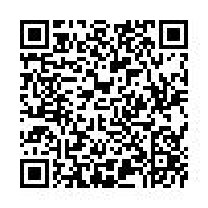
\includegraphics[width=0.3\textwidth]{img/QR/perfect_03.jpg}
  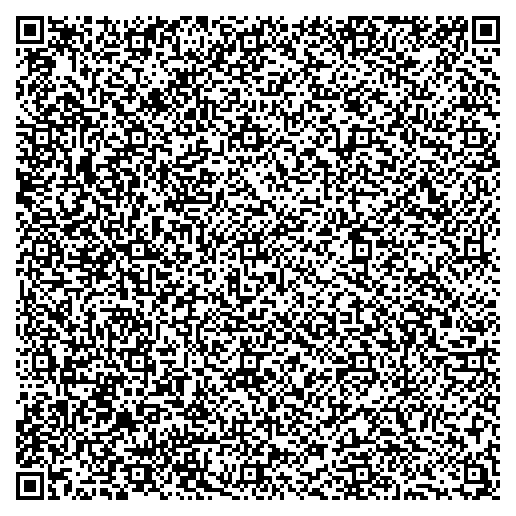
\includegraphics[width=0.3\textwidth]{img/QR/perfect_02.png}
  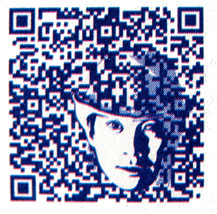
\includegraphics[width=0.3\textwidth]{img/QR/perfect_04.jpg}
  \caption{Normale Größe, groß, mit enthaltenem Bild}
  \label{fig:qrnormal}
\end{figure}
% \textbf{Bilder einfügen, (klein), normal, groß, (real), (dreckig), mit Bild}

% unscharfe
Auch Bilder, die mit einem Gaußschen Weichzeichner unscharf gemacht wurden, werden bis zu einem Radius von 3 Pixeln noch gut erkannt. Ab etwa 3,5 Pixeln sind die Kanten allerdings, wie in Abbildung \ref*{fig:qrblur} zu sehen ist, zu unscharf und der Code kann nicht dekodiert werden.
\begin{figure}[H]
  \centering
  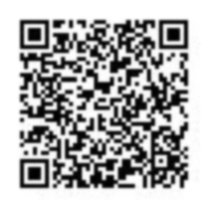
\includegraphics[width=0.3\textwidth]{img/QR/blurry_03_3.jpg}
  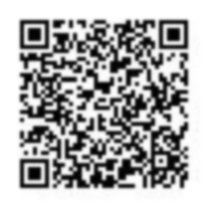
\includegraphics[width=0.3\textwidth]{img/QR/blurry_03_35f.jpg}
  \caption{Gaußscher Weichzeichner mit 3,0 Pixeln und 3,5 Pixeln Radius}
  \label{fig:qrblur}
\end{figure}
% \textbf{Bilder einfügen, blurry3, blurry35 }

% rotierte und rotiert+unscharf
In Abbildung \ref*{fig:qrrotate} sind rotierte QR-Codes abgebildet, dabei sieht man im ersten Bild eine 45$ ^\circ $ Drehung, da die Rotation des Bildes bei vollständigen QR-Codes unwichtig ist, das Bild wird immer akzeptiert. Allerdings können Fehler oder Überdeckungen dazu führen, dass Rotationen nur eingeschränkt durchführbar sind, wie z.B. beim Bild im Code(Bild 2/3), wo nur bis 25$^\circ$ und dann wieder ab 63$^\circ$ der Code erkannt wird.

Natürlich betrifft das auch unscharfe Bilder, die ebenfalls nicht bei jedem Drehwinkel erkannt werden. Das sieht man z.B. in Bild 4, wo mit 35$^\circ$ der Code noch erkannt wird, und in Bild 5, wo der um 40$^\circ$ gedrehte Code nicht mehr erkannt wird.
\begin{figure}[H]
  \centering
  \fbox{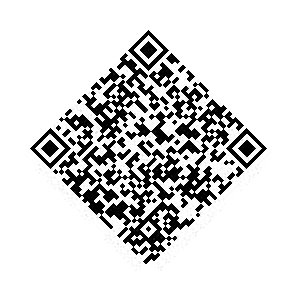
\includegraphics[width=0.3\textwidth]{img/QR/rotated_03_45.jpg}}
  \fbox{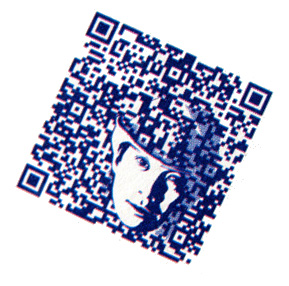
\includegraphics[width=0.3\textwidth]{img/QR/rotated_04_25.jpg}}
  \fbox{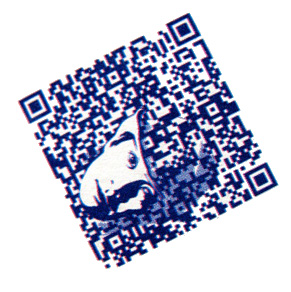
\includegraphics[width=0.3\textwidth]{img/QR/rotated_04_63.jpg}}
  \fbox{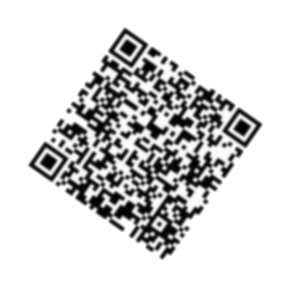
\includegraphics[width=0.3\textwidth]{img/QR/blurryrotate_03_3_35.jpg}}
  \fbox{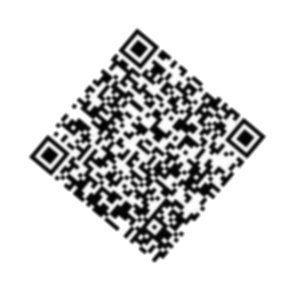
\includegraphics[width=0.3\textwidth]{img/QR/blurryrotate_03_3_40f.jpg}}
  \caption{Rotationen mit 45$^\circ$, 25$^\circ$, 63$^\circ$, 35$^\circ$ und 40$^\circ$}
  \label{fig:qrrotate}
\end{figure}
% \textbf{Bilder einfügen, rotate45, rotateface25, rotateface27f, rotateblurry35, rotateblurry40 }

% dunkle, dunkle+Fehler, dunkle+unscharf, dunkle+rotiert und dunkle+unscharf+rotiert
Die allgemeine Dunkelheit des Bildes, durch die der Kontrast sinkt, scheint kaum Auswirkungen auf die Erkennung der QR-Codes zu haben. Bei vollständigen Codes kann bis zu einer Abdunklung von 98\% immer noch der Code übersetzt werden, wobei selbst das menschliche Auge schon kaum noch etwas erkennen kann (siehe Abbildung \ref*{fig:qrdark}, Bild 1). Auch bei Codes mit integrierten Bildern ist, wie bei um 45$ ^\circ $ gedrehten Codes, eine Abdunklung bis zu 90\% kein Problem. Sogar bei maximal unscharfen und zusätzlich maximal gedrehten Codes ist eine Abdunklung von bis zu 90\% möglich, obwohl bei nur unscharfen Bildern scheinbar eine Grenze von 75\% besteht.
\begin{figure}[H]
  \centering
  
\includegraphics[width=0.3\textwidth]{img/QR/dark_03_98.jpg}
  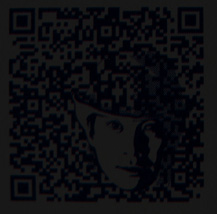
\includegraphics[width=0.3\textwidth]{img/QR/dark_04_90.jpg}
  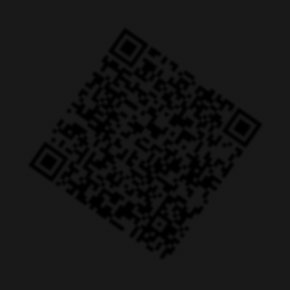
\includegraphics[width=0.3\textwidth]{img/QR/blurrydarkrotate_03_3_90_35.jpg}
  \caption{Dekodierbare Bilder: normal bei 98\%, mit Bild bei 90\% und rotiert+unscharf bei 90\% Abdunkelung}
  \label{fig:qrdark}
\end{figure}
% \textbf{Bilder einfügen, dark98, dark99f, darkface90, darkface95f, blurrydark75, blurrydark80f, blurrydarkrotate90, blurrydarkrotate95f }

% schatten
\todo{SCHATTEN}

% schräg
%SCHRÄG